\chapter{Phân Rã Ma Trận Và Trực Quan Hóa Với Manim}

\newpage

\section{Phân rã giá trị suy biến (SVD)}

\subsection{Định nghĩa ma trận SVD}

Phân rã giá trị suy biến - Singular Value Decomposition là một công cụ mạnh mẽ trong đại số tuyến tính, nó cho phép phân tích một ma trận bất kỳ $A \in \mathbb{R}^{m \times n}$ thành ba ma trận đặc biệt:

{\large
\begin{equation}
    A = U \Sigma V^T
\end{equation}
}

Trong đó:

\begin{itemize}[topsep=0pt, itemsep=2.5pt, leftmargin=1.5cm]
    \item $U \in \mathbb{R}^{m \times m}$: Là ma trận trực giao ($U^TU=I_{m}$), các cột của nó là các vector suy biến trái.
    \item $\Sigma \in \mathbb{R}^{m \times n}$: Là ma trận đường chéo không vuông, chứa các giá trị suy biến $\sigma_{i}$ trên đường chéo chính.
    \item $V^T \in \mathbb{R}^{n \times n}$: Là ma trận trực giao ($V^TV = I_{n}$), các cột của nó là các vector suy biến phải.
\end{itemize}

\subsection{Tính chất của các giá trị suy biến}

\textbf{Thứ tự và dấu}: Các giá trị suy biến luôn không âm và thường được sắp xếp giảm dần.

\begin{equation}
    \sigma_1 \geq \sigma_2 \geq \dots \sigma_p \geq 0 \text{ với } p = min(m, n)
\end{equation}

\textbf{Hạng ma trận}: Số lượng các giá trị suy biến khác 0 tương ứng với hạng của ma trận $A$.

\textbf{Xấp xỉ hạng thấp}: SVD cung cấp xấp xỉ tốt nhất cho ma trận ở hạng $k$ thấp hơn qua công thức $A_k = \Sigma_{i = 1}^{k} \sigma_i u_i v_i^T$, ứng dụng trong nén ảnh và khử nhiều.

\subsection{Mối liên hệ với giá trị riêng (Eigenvalues)}

SVD là sự tổng quát hóa của phép chéo hóa, có mối quan hệ chặt chẽ với các giá trị riêng của ma trận đối xứng:

\begin{itemize}[topsep=0pt, itemsep=2.5pt, leftmargin=1.5cm]
    \item \textbf{Công thức liên hệ}: Các giá trị suy biến $\sigma_i$ của $A$ là căn bậc hai của các giá trị riêng $\lambda_i$ của ma trận $A^TA$:

    \begin{equation}
        \sigma_i = \sqrt{\lambda_i(A^TA)}
    \end{equation}

    \item \textbf{Cơ sở vector}: Các cột của $V$ là các vector riêng của $A^TA$, trong khi các cột của $U$ là các vector riêng của $AA^T$.
\end{itemize}

\section{Ý nghĩa của phân rã SVD}

\subsection{Cơ chế hoạt động}

SVD không chỉ đơn thuần là một công thức đại số, về mặt bản chất nó chính là một chuỗi các phép biến đổi hình học cơ bản. Bất kỳ ma trận $A$ nào cũng được đại diện cho một phép biến đổi tuyến tính từ không gian $\mathbb{R}^m$ sang không gian $\mathbb{R}^n$.

SVD cho phép phân tách phép biến đổi này thành ba bước độc lập:

\begin{itemize}[topsep=0pt, itemsep=2.5pt, leftmargin=1.5cm]
    \item Phép xoay đầu tiên ($V^T$): Ma trận trực giao $V^T$ thực hiện xoay hệ tọa độ trong không gian sao cho các trục tọa độ ban đầu trùng với các vector suy biến phải ($v_{i}$). Bước này không làm thay đổi độ dài của các vector.
    \item Phép co giãn ($\Sigma$): Ma trận đường chéo $\Sigma$ thực hiện co giãn theo không gian dọc theo các trục tọa độ mới. Các vector sẽ được co giãn hoặc rút ngắn theo các hệ số $\sigma_i$. Nếu $\sigma_i$, chiều không gian tương ứng bị triệt tiêu, điều đó giải thích vì sao mà SVD có thể xác định được hạng (rank) và không gian null (nullspace).
    \item Phép xoay thứ hai ($U$): Ma trận trực giao $U$ xoay hệ tọa độ một lần nữa trong không gian để đưa các vector về vị trí cuối cùng theo các vector suy biến trái.
\end{itemize}

\begin{figure}[h]
    \vspace{0.75cm}
    \centering
    \scalebox{1}{
        \begin{minipage}{\textwidth}
            \centering
            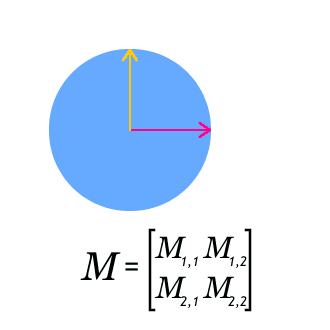
\includegraphics[width=0.25\textwidth]{images/chapter_02/svd-1.png}\hfill
            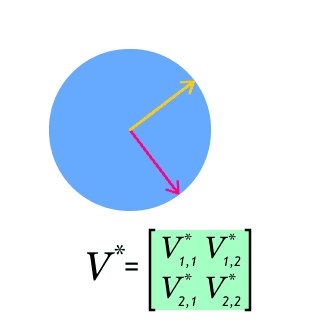
\includegraphics[width=0.25\textwidth]{images/chapter_02/svd-2.png}\hfill
            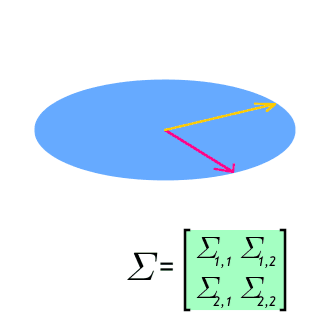
\includegraphics[width=0.25\textwidth]{images/chapter_02/svd-3.png}\hfill
            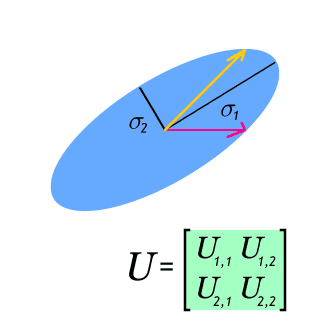
\includegraphics[width=0.25\textwidth]{images/chapter_02/svd-4.png}
        \end{minipage}
    }
    \caption{Các bước phân rã SVD}
    \label{fig:svd_decomp_steps}
\end{figure}

\newpage

\subsection{Vì sao cơ chế này quan trọng?}

Trong khi phép chéo hóa $A = PDP^{-1}$ chỉ hoạt động khi ta có thể tìm các trục mà tại đó ma trận chỉ thực hiện co giãn thì SVD chỉ ra rằng mọi ma trận (kể cả ma trận hình chữ nhật) đều có thể một cặp cơ sở trực chuẩn ($V$ và $U$) để biến hình cầu thành một hình ellipse.

Vì $U$ và $V$ là các ma trận trực giao, chúng không làm khuếch đại sai số tính toán làm cho thuật toán này trở nên ổn định nhất trong đại số tuyến tính. 

\section{Thuật toán giá trị riêng Jacobi}

\subsection{Định lý bất khả Abel}

Định lý phát biểu rằng \textbf{không tồn tại nghiệm đại số} - tức là nghiệm được biểu diễn bằng căn thức của phương trình đa thức tổng quát \textbf{bậc 5 hoặc lớn hơn} với các hệ số bất kỳ.

Trong quá trình tiến hành thuật toán SVD, chúng ta cần phải tìm các trị riêng của ma trận đối xứng $A^TA$. Việc tìm giá trị riêng tương đương với việc tìm nghiệm của đa thức đặc trưng $P(\lambda) = det(A - \lambda I) = 0$ nên đối với các ma trận có kích thước $\geq 5$, chúng ta không thể sử dụng các phương pháp đại số thông thường để giải quyết bài toán trên.

Dựa trên giới hạn của định lý Abel, ta phải sử dụng các phương pháp lặp số trị để giải quyết bài toán trên. Thuật toán Jacobi là lựa chọn tối ưu cho ma trận đối xứng vì:

\begin{itemize}[topsep=0pt, itemsep=2.5pt, leftmargin=1.5cm]
    \item Nó triệt tiêu các phần tử ngoài đường chéo bằng các phép xoay cho đến khi ma trận dần hội tụ về dạng đường chéo.
    \item Đảm bảo tính số học cao, phù hợp với yêu cầu ổn định số học của đồ án.
\end{itemize}

\newpage

\subsection{Chi tiết thuật toán}

\subsubsection{Phép xoay Jacobi}

Tại mỗi bước lặp, thuật toán chọn một phần tử ngoài đường chéo $s_{ij}$ (thường là phần tử có giá trị tuyệt đối lớn nhất) và triệt tiêu nó về 0 bằng một phép xoay trực giao, gọi là \textbf{ma trận xoay Jacobi} $G(i, j, \theta)$.

Ma trận $G$ giống với ma trận đơn vị nhưng có phần tử thay đổi tại bốn vị trí: $g_{ii}, g_{jj}, g_{ij} \text{ và } g_{ji}$. Khi đó, ma trận được cập nhật theo công thức: $S' = G^T S G$.

\begin{equation}
    \scalebox{0.9}{
    $
    G(i, j, \theta) = 
    \begin{bmatrix}
    1 &        &          & \text{\small Cột $i$} &        & \text{\small Cột $j$} &   \\
    & \ddots &          & \downarrow          &        & \downarrow                 &   \\
    &        & 1        &                     &        &                            &   \\
    &        &          & \cos\theta          & \dots  & -\sin\theta                & \rightarrow \text{\small Dòng $i$} \\
    &        &          & \vdots              & 1      & \vdots                     &   \\
    &        &          & \sin\theta          & \dots  & \cos\theta                 & \rightarrow \text{\small Dòng $j$} \\
    &        &          &                     &        & 1                          &   \\
    &        &          &                     &        &        & \ddots             &   \\
    &        &          &                     &        &        &                    & 1
    \end{bmatrix}
    $
    }
\end{equation}

Vì $G$ là ma trận trực giao nên phép biến đổi trên giữ nguyên đa thức đặc trưng của ma trận. Tức là $S$ và $S'$ có cùng tập hợp các trị riêng. Do đó mà ta có thể lặp lại quá trình mà vẫn giữ được các trị riêng ban đầu của $A^TA$.

Không những thế, ma trận trực giao $G$ có đặc tính bảo toàn bình phương tất cả các phần tử. Khi phép quay làm một phần tử ngoài đường chéo triệt tiêu về 0, giá trị đó không biến mất mà được "đẩy" vào các phần tử trên đường chéo chính.

\subsubsection{Tính toán góc xoay $\theta$}

Để phần tử $s_{ij}'$ trở về bằng $0$ sau phép biến đổi, góc $\theta$ được xác định dựa trên các phần tử hiện tại của ma trận $S$:

\begin{itemize}[topsep=0pt, itemsep=2.5pt, leftmargin=1.5cm]
    \item Nếu $s_{ii} = s_{jj}$ thì $\theta = \pi/4$.
    \item Nếu $s{ii} \neq s_{jj}$, ta tính $\theta$ thông qua giá trị $\tau = \frac{s_{jj} - s_{ii}}{2s_{ij}}$, sau đó tìm $t = tan(\theta)$ là nghiệm của phương trình $t^2 + 2rt - 1 = 0$.
\end{itemize}

\newpage

\subsubsection{Các bước thực hiện thuật toán}

\begin{algorithm}[H]
\caption{\textproc{Thuật toán trị riêng Jacobi}}
\begin{algorithmic}[1]
\Procedure{jacobi\_eigenvalues(A, $\epsilon$, max\_iter)}{}
    \State $S \gets A^TA$, $V \gets I_n$
    
    \State $is\_converge \gets False$

    \While{$is\_converge$}
        \State $max\_val \gets max(s_{ij}) \quad (i \neq j)$
        \If{$|s_{ij}| < \epsilon$ (với $\epsilon$ là ngưỡng sai số cực nhỏ)}
            \State $is\_converge \gets True$
            \State \textbf{break}
        \EndIf
        \State $cos(\theta), sin(\theta) \text{ được tính từ } s_{ii}, s_{jj}, s_{ij}$
        \State $S \gets G^T S G$ (ma trận $S$ dần trở thành ma trận đường chéo $\Sigma^2$)
        \State $V \gets V G$ (các cột của $V$ dần trở thành vector suy biến phải)
    \EndWhile
    \State $eigenvalues \gets \text{Các phần tử trên đường chéo chính của } S$
    \State \Return $eigenvalues, V$
\EndProcedure
\end{algorithmic}
\end{algorithm}

\newpage

\section{Chéo hóa ma trận}

\subsection{Cơ sở lý thuyết}

Một ma trận vuông $A \in \mathbb{R}^{n \times n}$ được gọi là chéo hóa được nếu tồn tại một ma trận khả nghịch $P$ và một ma trận đường chéo $D$ sao cho:

{\large
\begin{equation}
    A = PDP^{-1}
\end{equation}
}

Trong đó:

\begin{itemize}[topsep=0pt, itemsep=2.5pt, leftmargin=1.5cm]
    \item D là ma trận đường chéo $diag(\lambda_1, \lambda_2, \dots, \lambda_i)$ với $\lambda_i$ là các giá trị riêng của $A$.
    \item P là ma trận các vector riêng, trong đó mỗi cột của $P$ là một vector riêng ứng với giá trị riêng $\lambda_i$.
\end{itemize}

Quá trình chéo hóa phụ thuộc hoàn toàn vào việc tìm kiếm các đặc trưng phổ của ma trận:

\begin{itemize}[topsep=0pt, itemsep=2.5pt, leftmargin=1.5cm]
    \item \textbf{Trị riêng} $\lambda$: Trị riêng được xác định từ phương trình đặc trưng $det(A - \lambda I) = 0$. Đây là giá trị vô hướng thể hiện mức độ co giãn của ma trận theo một hướng nhất định.
    \item \textbf{Vector riêng} $x$: Vector riêng tương ứng là nghiệm của hệ $(A - \lambda I) = 0$. Nó đại diện cho hướng mà tại đó phép biến đổi tuyến tính chỉ đóng vai trò như phép nhân vô hướng.
    \item \textbf{Điều kiện chéo hóa}: Ma trận $A \in \mathbb{R}^{n \times n}$ chéo hóa được khi và chỉ khi tồn tại đủ $n$ vector riêng độc lập tuyến tính để cấu thành các cột của ma trận khả nghịch $P$.
\end{itemize}

\subsection{Trường hợp đặc biệt: Ma trận đối xứng thực}

\subsubsection{Định lý phổ (Spectral Theorem)}

Đối với ma trận vuông bất kỳ, việc chéo hóa được hay không phụ thuộc vào số lượng vector riêng độc lập tuyến tính. Tuy nhiên đối với ma trận đối xứng thực $A$, định lý phổ khẳng định:

\begin{itemize}[topsep=0pt, itemsep=2.5pt, leftmargin=1.5cm]
    \item $A$ \textbf{luôn} chéo hóa được.
    \item Tất cả các trị riêng của $A$ đều là \textbf{số thực}.
    \item Các vector riêng ứng với các giá trị riêng khác nhau của $A$ luôn \textbf{trực giao} với nhau.
\end{itemize}

\subsubsection{Chéo hóa trực giao}

Vì các vector riêng của ma trận đối xứng thực có thể chọn để tạo thành một bộ cơ sở trực chuẩn, công thức chéo hóa trở thành:

{\large
\begin{equation}
    A = QDQ^{-1}
\end{equation}
}

Trong đó:

\begin{itemize}[topsep=0pt, itemsep=2.5pt, leftmargin=1.5cm]
    \item $Q$ là ma trận trực giao thỏa mãn $Q^{-1} = Q^T$. Điều này giúp việc tính toán ma trận nghịch đảo trở nên đơn giản bằng một phép chuyển vị thay vì tốn chi phí $O(n^3)$ thông thường với ma trận $P$.
    \item $D$ là ma trận đường chéo chứa các trị riêng của $A$. 
\end{itemize}

\subsubsection{Vai trò và ý nghĩa trong tính toán}

\begin{itemize}[topsep=0pt, itemsep=2.5pt, leftmargin=1.5cm]
    \item \textbf{Sự ổn định}: Các phép biển đổi trực giao không làm khuếch đại sai số làm tròn, đảm bảo độ chính xác cực kỳ cao ($< 10^{-10}$) khi xử lý trong thực tế.
    \item \textbf{Mối liên hệ với SVD}: Đây là sự kết nối trực tiếp đến phân rã SVD. Trong SVD, chúng ta phải thực hiện chéo hóa ma trận đối xứng $A^TA$ để tìm các giá trị suy biến và vector suy biến phải. 
    \item \textbf{Tối ưu hiệu năng}: Đối với ma trận đối xứng xác định dương, chi phí tính toán có thể giảm xuống bằng một nửa so với các phương pháp thông thường.
\end{itemize}

\section{Phương pháp tìm trị riêng và vector riêng}

    

\newpage

\section{Trực quan hóa với Manim}